
%% $Id$

\chapter{Presenting theories}

Isabelle provides several ways to present the outcome of formal developments,
including WWW-based browsable libraries or actual printable documents.
Presentation is centered around the concept of \emph{logic sessions}.  The
global session structure is that of a tree, with Isabelle \texttt{Pure} at its
root, further object-logics derived (e.g.\ \texttt{HOLCF} from \texttt{HOL},
and \texttt{HOL} from \texttt{Pure}), and application sessions in leaf
positions.  The latter usually do not have a separate {\ML} image.

The \texttt{usedir} and \texttt{mkdir} utilities provide the prime means for
managing Isabelle sessions, including proper setup for presentation (see
\S\ref{sec:tool-usedir} and \S\ref{sec:tool-mkdir}).


\section{Generating theory browsing information} \label{sec:info}
\index{theory browsing information|bold}

As a side-effect of running a logic sessions, Isabelle is able to generate
theory browsing information, including HTML documents that show a theory's
definition, the theorems proved in its ML file and the relationship with its
ancestors and descendants.  Besides the HTML file that is generated for every
theory, Isabelle stores links to all theories in an index file. These indexes
are linked with other indexes to represent the overall tree structure of logic
sessions.

Isabelle also generates graph files that represent the theory hierarchy of a
logic.  There is a graph browser Java applet embedded in the generated HTML
pages, and also a stand-alone application that allows browsing theory graphs
without having to start a WWW browser first.  The latter version also includes
features such as generating {\sc PostScript} files, which are not available in
the applet version.  See \S\ref{sec:browse} for further information.

\medskip

In order to let Isabelle generate theory browsing information, simply append
``\texttt{-i true}'' to the \settdx{ISABELLE_USEDIR_OPTIONS} setting before
making a logic.  For example, in order to do this for {\FOL}, add this to your
Isabelle settings file
\begin{ttbox}
ISABELLE_USEDIR_OPTIONS="-i true"
\end{ttbox}
and then change into the \texttt{src/FOL} directory of the Isabelle
distribution and run \texttt{isatool make}, or even \texttt{isatool make all}.

Some sessions (such as \texttt{HOL/Isar_examples}) even provide actual
printable documents.  These are prepared automatically as well if enabled like
this, using the \texttt{-d} option
\begin{ttbox}
ISABELLE_USEDIR_OPTIONS="-i true -d dvi"
\end{ttbox}
See \S\ref{sec:tool-document} for further information on Isabelle document
preparation.

\bigskip The theory browsing information is stored within the directory
determined by the \settdx{ISABELLE_BROWSER_INFO} setting.  The
\texttt{index.html} file located there provides an entry point to all standard
Isabelle logics.  A complete HTML version of all object-logics and examples of
the Isabelle distribution is available at
\begin{center}\small
  \begin{tabular}{l}
    \url{http://www.cl.cam.ac.uk/Research/HVG/Isabelle/library/} \\
    \url{http://isabelle.in.tum.de/library/} \\
  \end{tabular}
\end{center}

\medskip

The generated HTML document of any theory includes all theorems proved in the
corresponding {\ML} file, provided these have been stored properly via
\ttindex{qed}, \ttindex{qed_goal}, \ttindex{qed_goalw}, \ttindex{bind_thm},
\ttindex{bind_thms} or \ttindex{store_thm} (see also \cite{isabelle-ref}).
Section headings may be included in the presentation via the {\ML} function
\begin{ttbox}\index{*section}
section: string -> unit
\end{ttbox}

\medskip

In order to present your own theories on the web, simply copy the whole
\texttt{ISABELLE_BROWSER_INFO} directory to your WWW server, after generating
browser info like this:
\begin{ttbox}
isatool usedir -i true HOL Foo
\end{ttbox}
This assumes that directory \texttt{Foo} contains some \texttt{ROOT.ML} file
to load all your theories, and {\HOL} is your parent logic image.  Ideally,
theory browser information would have been generated for {\HOL} already.

Alternatively, one may specify an external link to an existing body of HTML
data by giving \texttt{usedir} a \texttt{-P} option like this:
\begin{ttbox}
isatool usedir -i true -P http://isabelle.in.tum.de/library/ HOL Foo
\end{ttbox}

\medskip For production use, the \texttt{usedir} tool is usually invoked in an
appropriate \texttt{IsaMakefile}, via the Isabelle \texttt{make} utility.
There is a separate \texttt{mkdir} tool to provide easy setup of all this,
with only minimal manual editing required.
\begin{ttbox}
isatool mkdir -d Foo
edit Foo/ROOT.ML
isatool make
\end{ttbox}
See \S\ref{sec:tool-mkdir} for more information on preparing Isabelle session
directories, including the setup for documents.


\section{Browsing theory graphs} \label{sec:browse}
\index{theory graph browser|bold} 

The graph browser is a tool for visualizing dependency graphs. Certain nodes
of the graph (i.e.~theories) can be grouped together in ``directories'', whose
contents may be hidden, thus enabling the user to filter out irrelevant
information.  The browser is written in Java, it can be used both as a
stand-alone application and as an applet.


\subsection{Invoking the graph browser}

The stand-alone version of the graph browser is wrapped up as an
Isabelle tool called \tooldx{browser}:
\begin{ttbox}
Usage: browser [GRAPHFILE]
\end{ttbox}
When no filename is specified, the browser automatically changes to
the directory \texttt{ISABELLE_BROWSER_INFO/graph/data}.

\medskip The applet version of the browser can be invoked by opening the {\tt
  index.html} file in the directory \texttt{ISABELLE_BROWSER_INFO} from your
Web browser and selecting the version ``including theory graph browser''.
There is also a link to the corresponding theory graph in every logic's {\tt
  index.html} file.


\subsection{Using the graph browser}

The browser's main window, which is shown in figure
\ref{browserwindow}, consists of two sub-windows: In the left
sub-window, the directory tree is displayed. The graph itself is
displayed in the right sub-window.
\begin{figure}[ht]
  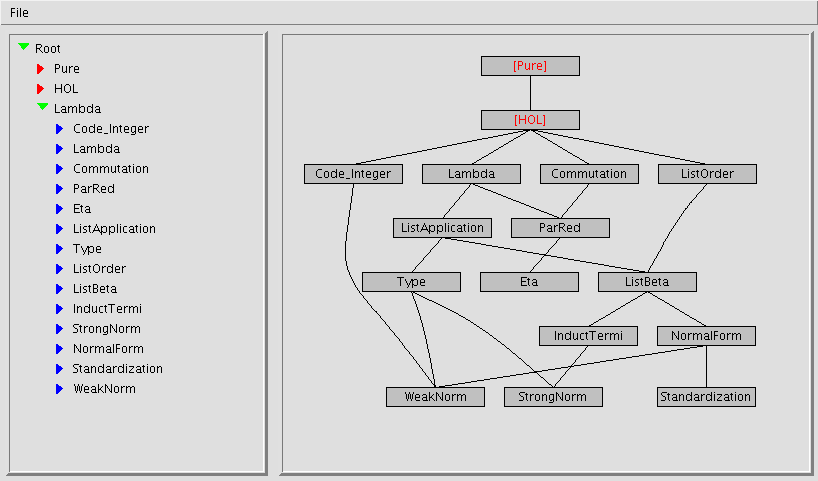
\includegraphics[width=\textwidth]{browser_screenshot}
  \caption{\label{browserwindow} Browser main window}
\end{figure}


\subsubsection*{The directory tree window}

We describe the usage of the directory browser and the meaning of the
different items in the browser window.
\begin{itemize}
  
\item A red arrow before a directory name indicates that the directory
  is currently ``folded'', i.e.~the nodes in this directory are
  collapsed to one single node. In the right sub-window, the names of
  nodes corresponding to folded directories are enclosed in square
  brackets and displayed in red color.
  
\item A green downward arrow before a directory name indicates that
  the directory is currently ``unfolded''. It can be folded by
  clicking on the directory name.  Clicking on the name for a second
  time unfolds the directory again.  Alternatively, a directory can
  also be unfolded by clicking on the corresponding node in the right
  sub-window.
  
\item Blue arrows stand before ordinary node names. When clicking on such a
  name (i.e.\ that of a theory), the graph display window focuses to the
  corresponding node. Double clicking invokes a text viewer window in which
  the contents of the theory file are displayed.

\end{itemize}


\subsubsection*{The graph display window}

When pointing on an ordinary node, an upward and a downward arrow is
shown.  Initially, both of these arrows are green. Clicking on the
upward or downward arrow collapses all predecessor or successor nodes,
respectively. The arrow's color then changes to red, indicating that
the predecessor or successor nodes are currently collapsed. The node
corresponding to the collapsed nodes has the name ``{\tt [....]}''. To
uncollapse the nodes again, simply click on the red arrow or on the
node with the name ``{\tt [....]}''. Similar to the directory browser,
the contents of theory files can be displayed by double clicking on
the corresponding node.


\subsubsection*{The ``File'' menu}

Please note that due to Java security restrictions this menu is not
available in the applet version. The meaning of the menu items is as
follows:
\begin{description}
  
\item[Open \dots] Open a new graph file.
  
\item[Export to PostScript] Outputs the current graph in {\sc
    PostScript} format, appropriately scaled to fit on one single
  sheet of paper.  The resulting file can be printed directly.
  
\item[Export to EPS] Outputs the current graph in Encapsulated {\sc
    PostScript} format. The resulting file can be included in other
  documents.

\item[Quit] Quit the graph browser.

\end{description}


\subsection*{*Syntax of graph definition files}

A graph definition file has the following syntax:
\begin{eqnarray*}
  \mbox{\it graph} & = & \{ \: \mbox{\it vertex \tt ;} \: \} ^ + \\
  vertex & = & \mbox{\it vertexname} \: \mbox{\it vertexID} \: \mbox{\it dirname} \: [ \mbox{\tt +} ]
  \: \mbox{\it path} \: [ \mbox{\tt <} | \mbox{\tt >} ] \: \{ \: \mbox{\it vertexID} \: \} ^ *
\end{eqnarray*}

The meaning of the items in a vertex description is as follows:
\begin{description}
  
\item[vertexname] The name of the vertex.
  
\item[vertexID] The vertex identifier. Note that there may be two
  vertices with equal names, whereas identifiers must be unique.
  
\item[dirname] The name of the ``directory'' the vertex should be
  placed in.  A ``{\tt +}'' sign after {\it dirname} indicates that
  the nodes in the directory are initially visible. Directories are
  initially invisible by default.
  
\item[path] The path of the corresponding theory file. This is
  specified relatively to the path of the graph definition file.
  
\item[List of successor/predecessor nodes] A ``{\tt <}'' sign before
  the list means that successor nodes are listed, a ``{\tt >}'' sign
  means that predecessor nodes are listed. If neither ``{\tt <}'' nor
  ``{\tt >}'' is found, the browser assumes that successor nodes are
  listed.

\end{description}


\section{Preparing Isabelle session documents --- \texttt{isatool document}}
\label{sec:tool-document}

The \tooldx{document} utility prepares logic session documents, processing the
sources both as provided by the user and generated by Isabelle.  Its usage is:
\begin{ttbox}
Usage: document [OPTIONS] [DIR]

  Options are:
    -c           remove DIR after succesful run (!)
    -o FORMAT    specify output format: dvi (default), dvi.gz, ps,
                 ps.gz, pdf

  Prepare the theory session document in DIR (default 'document')
  producing the specified output format.
\end{ttbox}
This tool is usually run automatically as part of the corresponding session,
provided document preparation has been enabled (cf.\ the \texttt{-d} option of
the \texttt{usedir} utility, \S\ref{sec:tool-usedir}).  It may be manually
invoked on the generated browser information document output as well.

\medskip Document preparation requires a properly setup ``\texttt{document}''
directory within the logic session sources.  This directory is supposed to
contain all the files needed to produce the final document --- apart from the
actual theories which are generated by Isabelle.

\medskip For simple documents, the \texttt{document} tool is smart enough to
create any of the output formats, taking \texttt{root.tex} supplied by the
user as a starting point.  This even includes multiple runs of {\LaTeX} to
accommodate references and bibliographies (the latter assumes
\texttt{root.bib} within the same directory).

For complex documents, a separate \texttt{IsaMakefile} may be given instead.
It should provide targets for any admissible document format; these have to
produce corresponding output files named after \texttt{root} as well, e.g.\ 
\texttt{root.dvi} for target format \texttt{dvi}.

\medskip When running the session, Isabelle copies the original
\texttt{document} directory into its proper place within
\texttt{ISABELLE_BROWSER_INFO} according to the session path.  Then, for any
processed theory $A$ some {\LaTeX} source is generated and put there as
$A$\texttt{.tex}.  Furthermore, a list of all generated theory files is put
into \texttt{session.tex}.  Typically, the root {\LaTeX} file provided by the
user would include \texttt{session.tex} to get a document containing all the
theories.

The {\LaTeX} versions of the theories require some macros defined in
\texttt{isabelle.sty} as distributed with Isabelle.  Doing
\verb,\usepackage{isabelle}, somewhere in \texttt{root.tex} should work fine;
the underlying Isabelle \texttt{latex} utility already includes an appropriate
{\TeX} inputs path.

If the text contains any references to Isabelle symbols (such as
\verb,\<forall>,) then \texttt{isabellesym.sty} should be included as well.
This package contains a standard set of {\LaTeX} macro definitions
\verb,\isasym,$foo$ corresponding to \verb,\<,$foo$\verb,>,.  The user may
refer to further symbols as well, simply by providing {\LaTeX} macros of the
same sort.

For proper setup of PDF documents (with hyperlinks, bookmarks, and thumbnail
images), we recommend to include \verb,pdfsetup.sty, as well.  It is safe to
do so even without using PDF~\LaTeX.

\medskip As a final step, \texttt{isatool document -c} is run on the resulting
\texttt{document} directory.  Thus the actual output document is built and
installed in its proper place (as linked by the session's
\texttt{index.html}).  The generated sources are deleted after successful run
of {\LaTeX} and friends.  Note that a copy of the sources may be retained by
passing an option \texttt{-D} to the \texttt{usedir} utility when running the
session (see also \S\ref{sec:tool-usedir}).


\section{Running {\LaTeX} within the Isabelle environment --- \texttt{isatool latex}}
\label{sec:tool-latex}

The \tooldx{latex} utility provides the basic interface for Isabelle document
preparation.  Its usage is:
\begin{ttbox}
Usage: latex [OPTIONS] [FILE]

  Options are:
    -o FORMAT    specify output format: dvi (default), dvi.gz, ps,
                 ps.gz, pdf, bbl, png, sty

  Run LaTeX (and related tools) on FILE (default root.tex),
  producing the specified output format.
\end{ttbox}
Appropriate {\LaTeX}-related programs are run on the input file, according to
the given output format: \texttt{latex}, \texttt{pdflatex}, \texttt{dvips},
\texttt{bibtex} (for \texttt{bbl}), and \texttt{thumbpdf} (for \texttt{png}).
The actual commands are determined from the settings environment
(\texttt{ISABELLE_LATEX} etc., see \S\ref{sec:settings}).

The \texttt{sty} output format causes the Isabelle style files to be updated
from the distribution.  This is useful in special situations where the
document sources are to be processed another time by separate tools (cf.\ 
option \texttt{-D} of the \texttt{usedir} utility, see
\S\ref{sec:tool-usedir}).

It is important to note that the {\LaTeX} inputs file space has to be properly
setup to include the Isabelle styles.  Usually, this may be done by modifying
the \settdx{TEXINPUTS} variable in settings like this:
\begin{ttbox}
TEXINPUTS="$ISABELLE_HOME/lib/texinputs:$TEXINPUTS"
\end{ttbox}
This is known to work with recent versions of the \textsl{teTeX} distribution.


\section{Creating Isabelle session directories --- \texttt{isatool mkdir}}
\label{sec:tool-mkdir}

The \tooldx{mkdir} utility prepares Isabelle session source directories,
including a sensible default setup of \texttt{IsaMakefile}, \texttt{ROOT.ML}
and an optional \texttt{document} directory.  Its usage is:
\begin{ttbox}
Usage: mkdir [LOGIC] NAME

  Options are:
    -I FILE      alternative IsaMakefile output
    -P           include parent logic target
    -b           setup build mode (session outputs heap image)
    -d           setup document

  Prepare session directory, including IsaMakefile, document etc.
  with parent LOGIC (default ISABELLE_LOGIC=\$ISABELLE_LOGIC)
\end{ttbox}

The \texttt{mkdir} tool is conservative in the sense that any existing
\texttt{IsaMakefile} etc.\ is left unchanged.  Thus it is safe to invoke it
experimentally, with varying options.

Note that \texttt{mkdir} is unable to change \texttt{IsaMakefile}
incrementally --- manual changes are required for multiple sub-sessions.  On
order to get an initial working session, the only editing needed is to add
appropriate \texttt{use_thy} calls to the generated \texttt{ROOT.ML} file.


\subsection*{Options}

The \texttt{-I} option specifies an alternative to \texttt{IsaMakefile} for
dependencies.  Note that ``\texttt{-}'' refers to \emph{stdout}, i.e.\ 
``\texttt{-I-}'' provides an easy way to peek at \texttt{mkdir}'s idea of
\texttt{make} setup required for some particular of Isabelle session.

\medskip The \texttt{-P} option includes a target for the parent
\texttt{LOGIC} session in the generated \texttt{IsaMakefile}.  The
corresponding sources are assumed to be located within the Isabelle
distribution.

\medskip The \texttt{-b} option sets up the current directory as the base for
a new session that provides an actual logic image, as opposed to one that only
runs several theories based on an existing image.  Note that in the latter
case, everything except \texttt{IsaMakefile} would be placed into a separate
directory \texttt{NAME}, rather than the current one.  See
\S\ref{sec:tool-usedir} for further information on \emph{build mode} vs.\ 
\emph{example mode} of the \texttt{usedir} utility.

\medskip The \texttt{-d} option creates a \texttt{document} directory with a
minimal \texttt{root.tex} file, which is sufficient to get all theories pretty
printed in the order of appearance.  See \S\ref{sec:tool-document} for further
information on Isabelle document preparation.


\subsection*{Examples}

The standard setup of a single ``example session'' based on the default logic,
with proper document generation is generated like this:
\begin{ttbox}
isatool mkdir -d Foo
\end{ttbox}
\noindent The theory sources should be put into the \texttt{Foo} directory, and its
\texttt{ROOT.ML} should be edited to load all required theories.  Invoking
\texttt{isatool make} would now run the whole session, generating browser
information and the document automatically.  The \texttt{IsaMakefile} is
usually tuned manually later, e.g.\ adding actual source dependencies, or
changing the options passed to \texttt{usedir}.


\section{Running Isabelle sessions --- \texttt{isatool usedir}} \label{sec:tool-usedir}

The \tooldx{usedir} utility builds object-logic images, or runs example
sessions based on existing logics. Its usage is:
\begin{ttbox}
Usage: usedir LOGIC NAME

  Options are:
    -D PATH      dump generated document sources into PATH
    -P PATH      set path for remote theory browsing information
    -b           build mode (output heap image, using current dir)
    -c BOOL      tell ML system to compress output image (default true)
    -d FORMAT    build document as FORMAT (default false)
    -i BOOL      generate theory browsing information,
                 i.e. HTML / graph data (default false)
    -r           reset session path
    -s NAME      override session NAME

  Build object-logic or run examples. Also creates browsing
  information (HTML etc.) according to settings.

  ISABELLE_USEDIR_OPTIONS=
\end{ttbox}

Note that the value of the \settdx{ISABELLE_USEDIR_OPTIONS} setting is
implicitly prefixed to \emph{any} \texttt{usedir} call. Since the
\ttindex{IsaMakefile}s of all object-logics distributed with Isabelle just
invoke \texttt{usedir} for the real work, one may control compilation options
globally via above variable. In particular, generation of \rmindex{HTML}
browsing information and document preparation is controlled here.


\subsection*{Options}

Basically, there are two different modes of operation: \emph{build mode}
(enabled through the \texttt{-b} option) and \emph{example mode} (default).

Calling \texttt{usedir} with \texttt{-b} runs \texttt{isabelle} with input
image \texttt{LOGIC} and output to \texttt{NAME}, as provided on the command
line. This will be a batch session, running \texttt{ROOT.ML} from the current
directory and then quitting.  It is assumed that \texttt{ROOT.ML} contains all
{\ML} commands required to build the logic.

In example mode, \texttt{usedir} runs a read-only session of \texttt{LOGIC}
and automatically runs \texttt{ROOT.ML} from within directory \texttt{NAME}.
It assumes that this file contains appropriate {\ML} commands to run the
desired examples.

\medskip The \texttt{-i} option controls theory browser data generation. It
may be explicitly turned on or off --- as usual, the last occurrence of
\texttt{-i} on the command line wins.  The \texttt{-P} option specifies a path
(or actual URL) to be prefixed to any \emph{non-local} reference of existing
theories.  Thus user sessions may easily link to existing Isabelle libraries
already present on the WWW.

\medskip The \texttt{-d} option controls document preparation.  Valid
arguments are \texttt{false} (do not prepare any document; this is default),
or any of \texttt{dvi}, \texttt{dvi.gz}, \texttt{ps}, \texttt{ps.gz},
\texttt{pdf}.  The logic session has to provide a properly setup
\texttt{document} directory.  See \S\ref{sec:tool-document} and
\S\ref{sec:tool-latex} for more details.

\medskip The \texttt{-D} option causes the generated document sources to be
dumped at location \texttt{PATH}, which is relative to the session's main
directory.  For example, \texttt{-D document} would leave a copy of the
{\LaTeX} sources in the actual document directory.  Thus the Isabelle
\texttt{document} or \texttt{latex} tools may be run later, facilitating much
easier debugging of {\LaTeX} errors, for example.  Note that a copy of the
Isabelle style files will be placed in \texttt{PATH} as well.

\medskip Any \texttt{usedir} session is named by some \emph{session
  identifier}. These accumulate, documenting the way sessions depend on
others. For example, consider \texttt{Pure/FOL/ex}, which refers to the
examples of {\FOL}, which in turn is built upon {\Pure}.

The current session's identifier is by default just the base name of the
\texttt{LOGIC} argument (in build mode), or of the \texttt{NAME} argument (in
example mode). This may be overridden explicitly via the \texttt{-s} option.


\subsection*{Examples}

Refer to the \texttt{IsaMakefile}s of the Isabelle distribution's
object-logics as a model for your own developments.  For example, see
\texttt{src/FOL/IsaMakefile}.  The Isabelle \texttt{mkdir} tool (see
\S\ref{sec:tool-mkdir}) creates \texttt{IsaMakefile}s with proper invocation
of \texttt{usedir} as well.


%%% Local Variables: 
%%% mode: latex
%%% TeX-master: "system"
%%% End: 
